\documentclass{beamer}
\usepackage[utf8]{inputenc}

\author[Sowmya Vajjala]{Instructor: Sowmya Vajjala}


\title[LING 120]{LING 120, Fall 2017: \\ Language and Computers}
\subtitle{Topic: Overview of Natural Language Processing}

\date{2 October 2017 (Week 7)}

\institute{Iowa State University, USA}

\usepackage{graphicx}
%%%%%%%%%%%%%%%%%%%%%%%%%%%

\begin{document}

\begin{frame}\titlepage
\end{frame}

\begin{frame}%2minutes
\frametitle{Class outline}
\begin{itemize}
\item Reminders, Announcements etc.
\item Natural Language Processing: What is it, and why now?
\item Examples of bottlenecks in automatically understanding human language
\item Tasks in NLP: an overview
\end{itemize}
\end{frame}

\begin{frame}
\frametitle{Reminders and Announcements}
\begin{itemize}
\item Assignment 3 is due this week! (7th October) \pause 
\item Midterm related stuff:
\begin{itemize}
\item Presentations are due next week (3 teams on Monday, 3 on Wednesday)
\item You can get your laptops or use mine (If you use mine, send a PDF - I don't have powerpoint)
\item Suggestion: Do the presentations using Google slides or some such collaborative online tool.
\item I will accomodate some time in the class on Wednesday (and may be Friday) for this. 
\end{itemize} \pause
\item Assignment 4: description in Friday's class
\end{itemize}
\end{frame}

\begin{frame}
\frametitle{What is NLP? and Why now?}
\begin{itemize}
\item What: It is a field concerned with the interaction between computers and human languages. 
\item Address issues like - how can computers process and understand large amounts of data in various human languages. \pause
\item In Week 1, I gave an overview of where is Language understanding is relevant in real life computer based applications. 
\item Now that you gained some knowledge of different applications of language, it is time to think about those initial questions again, in more detail. 
\end{itemize}
\end{frame}

%2 slides from week 1:
\begin{frame}
\frametitle{Example from Week 1}
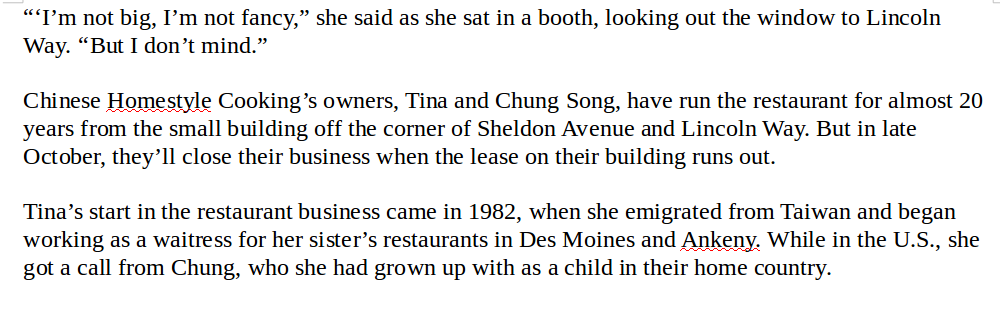
\includegraphics[width=0.9\textwidth]{Example.png}
\\ \footnotesize{Source: Ames Tribune (\url{http://goo.gl/zvx9Uw})}

\begin{enumerate}
\item When she says "I" in the first sentence, does she mean herself literally? 
\item What is she referring to? When will we know what is she referring to?
\item Who is "She"?
\item What is "Chinese Homestyle Cooking" referring to?
\end{enumerate}
\end{frame}

\begin{frame}
\frametitle{More Questions}
\frametitle{Let us take a small text snippet -2}
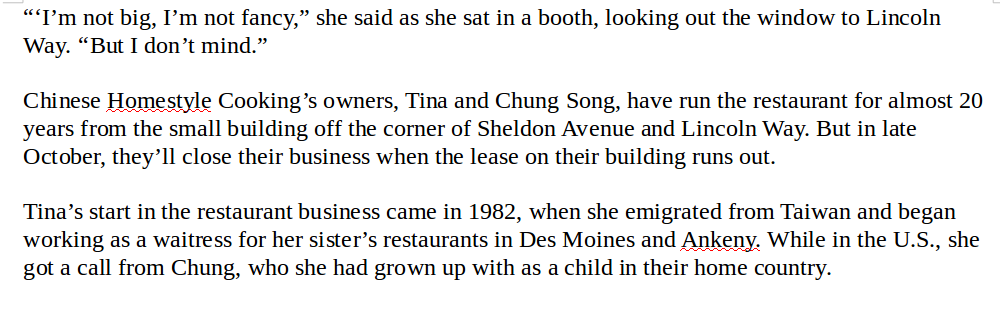
\includegraphics[width=0.9\textwidth]{Example.png}
\\ \footnotesize{Source: Ames Tribune \url{http://goo.gl/zvx9Uw}}
\begin{enumerate}
\item What is the main event of this text?
\item What is the relationship between "Chinese Homestyle cooking" and Tina?
\item Is Lincoln Way something related to President Lincoln?
\end{enumerate}
\end{frame}


\begin{frame}
\frametitle{}
\Large So, what is it about language that makes it difficult for a computer to process the text and answer such questions?
\end{frame}

\begin{frame}
\frametitle{1. Language is ambiguous}
\framesubtitle{Some ambiguous sentences}
\begin{itemize}
\item Newspaper headlines
\begin{itemize}
\item "Children make delicious snacks"
\item "Dead expected to rise"
\item "Republicans grill IRS chief over lost emails"
\end{itemize}
\item Normal, grammatical sentences can be ambiguous too:
\begin{itemize}
\item "I saw a man on a hill with a telescope."
\item "Look at the man with one eye"
\end{itemize}
\end{itemize}
We are not even talking about ambiguities involving speech or alternative interpretations due to stress/emphasis on some word.
\end{frame}

\begin{frame}
\frametitle{Some types of ambiguity}
\begin{enumerate}
\item Lexical ambiguity: due to multiple meanings or senses of word usage
\\ e.g., He stood near the \textbf{bank} \pause
\item Structural ambiguity: due to syntactic structure
\\ e.g., I saw the man on the hill with telescope. \pause
\item Semantic ambiguity: more interpretations possible
\\ e.g., John and Mary are married (to each other? or to different people?) \pause
\item Referential ambiguity
\\ e.g., She dropped the \textit{plate} on the \textit{table} and broke \textbf{it} \pause
\item Ambiguity due to the use of non-literal language
\\ e.g., Time flies like an arrow
\end{enumerate}
Good source to read more: \url{http://cs.nyu.edu/faculty/davise/ai/ambiguity.html}
\end{frame}

\begin{frame}
\frametitle{Ambiguity for humans}
\framesubtitle{personal experience}
\begin{itemize}
\item "ISU sends out alert as devastating weed spreads in Iowa" - read a local newspaper headline last year. What did you understand?
\pause
\item My immediate reaction: Some new drug is circulating and ISU wants its students to be aware and not consume it. 
\pause
\item However, the actual news is about some poisonous wild plant, and the alert was issued by ISU weed and crop specialists to farmers.
\end{itemize}
... so some humans also cannot disambiguate certain things, due to... may be.. cultural differences?
\end{frame}

\begin{frame}
\frametitle{2. "common" knowledge for humans}
Look at these two sentences:
\\ Dog bit man.
\\ Man bit dog.
\\ - For a computer, both of them are linguistically the same. We know only the first one is "normal" English sentence (I hope!) because we have "world knowledge".
\end{frame}

\begin{frame}
\frametitle{3. Language is creative}
Literary texts have their own language style: long sentences, neologisms, creative usage of words etc.
\end{frame}

\begin{frame}
\frametitle{4. Language can be complex to understand}
Legal documents, Writing style of some authors, propaganda materials, etc.
\end{frame}

\begin{frame}
\frametitle{5. Language is Diverse}
\framesubtitle{Some Examples}
\begin{itemize}
\item There are different types of text online: news, tweets, SMS, email, forum posts, speech transcripts etc.
\item Each genre has some specific characteristics of its own
\item NLP methods should generalize to all genres, and at the same time capture such specific characteristics
\item Example: a machine translation model created by training examples from European parliament speeches should also be able to translate casual day to day conversations.
\end{itemize}
\end{frame}

\begin{frame}
\frametitle{6. Other Issues}
\begin{itemize}
\item different text formats (pdf, doc, txt etc)
\item spelling variations
\item sarcasm
\item slang
\item using synonyms, paraphrases etc 
\end{itemize}
.. and so on.
\end{frame}

\begin{frame}
\frametitle{7. Languages are many}
.. and each language has its own special characteristics apart from similarities with other languages. NLP should handle both these aspects. 
\end{frame}

\begin{frame}
\frametitle{}
\Large Tasks in NLP: An overview
\end{frame}


\begin{frame}
\frametitle{NLP tasks: Word Collocations and Concordances}
\begin{itemize}
\item Task: compiling lists of words, or word sequences occuring in documents.
\item Simplest and least ambiguous form of language processing. 
\item Can get to more advanced collocations beyond surface forms.
\item Established methods exist for collecting different kinds of collocations
\end{itemize}
\end{frame}

\begin{frame}
\frametitle{NLP tasks: Pattern Extraction}
\begin{itemize}
\item Task: Extract the language patterns that exist in textual data. 
\item Regular expressions are very useful for this
\item More advanced methods (which rely on machine learning) exist to extract unknown patterns from unstructured text documents.
\end{itemize}
\end{frame}

\begin{frame}
\frametitle{NLP tasks: POS Tagging}
\framesubtitle{What is the big deal about automatic tagging?}
\begin{itemize}
\item Task: Given a sequence of words, return the POS tags for each word.
\item An example problem: What is the best tag for a word in a context?
\begin{itemize}
\item I wish to cite this work. 
\\ PRP/I  VBP/wish  TO/to  VB/cite  DT/this  NN/work ./.
\item He has a wish.
\\ PRP/He  VBZ/has  DT/a  NN/wish ./. 
\end{itemize}
\item Largely considered solved for English, but there are still issues if we go beyond typical newspaper language (e.g., tagging speech or tweets). Still an unsolved problem for several languages.
\end{itemize}
(to be continued)
\end{frame}

\begin{frame}
\frametitle{Attendance Exercise}
\begin{itemize}
\item Form into your mid-term teams, do the exercise in the given worksheet, write the names of your teammates and return to me.
\item This counts as your attendance for today. 
\item Source: \url{http://www.nacloweb.org/resources/problems/2011/E.pdf}
\end{itemize}
\end{frame}

\end{document}


%Friday question: sentiment analysis - NACLO question or just showing a few movie reviews and asking them about positive or neg sentiment, how a computer does it, etc.

